\section{Análise de Desempenho por Classe}

Embora as métricas globais forneçam uma visão geral da eficácia de cada modelo, uma análise detalhada por categoria é fundamental para diagnosticar a confiabilidade do sistema de classificação de algodão. Nesta seção, detalhamos o desempenho da arquitetura campeã, a \textbf{DenseNet (V10)}, desmembrando suas métricas por classe.

A Tabela \ref{tab:best_class_metrics} apresenta a precisão, revocação e o escore F1 para cada uma das 10 classes presentes no dataset de teste. Nota-se que o modelo demonstra um desempenho excepcional em classes como \textbf{44.4} (F1 de 0,883) e \textbf{32.3} (F1 de 0,806). Em contrapartida, as classes de transição morfológica como a \textbf{41.4} apresentaram os maiores desafios, com revocação de apenas 0,407.

\begin{table}[!h]
    \centering
    \begin{threeparttable}
    \caption{Análise de desempenho por classe do melhor modelo (DenseNet V10).}
    \label{tab:best_class_metrics}
    \begin{tabular}{llll}
\toprule
 & Precisão & Revocação & Escore F1 \\
\midrule
31.2 & 0,628 & 0,744 & 0,681 \\
31.3 & 0,529 & 0,455 & 0,489 \\
31.4 & 0,492 & 0,547 & 0,518 \\
32.3 & 0,551 & 0,674 & 0,607 \\
32.4 & 0,778 & 0,406 & 0,533 \\
33.3 & 0,617 & 0,579 & 0,598 \\
41.4 & 0,619 & 0,441 & 0,515 \\
41.5 & 0,724 & 0,724 & 0,724 \\
42.4 & 0,673 & 0,434 & 0,528 \\
44.4 & 0,769 & 0,698 & 0,732 \\
\bottomrule
\end{tabular}

    \begin{tablenotes}
            \small 
            \item[] Fonte: Do autor.
        \end{tablenotes}
        \end{threeparttable}
\end{table}

Para diagnóstico qualitativo dos erros, a Matriz de Confusão Normalizada para a DenseNet V10 é apresentada na Figura \ref{fig:matriz_confusao_final}. A diagonal principal representa a taxa de acerto (\textit{recall}) para cada classe, enquanto os valores fora da diagonal indicam a proporção e o padrão das classificações incorretas.

\begin{figure}[h!]
  \centering
  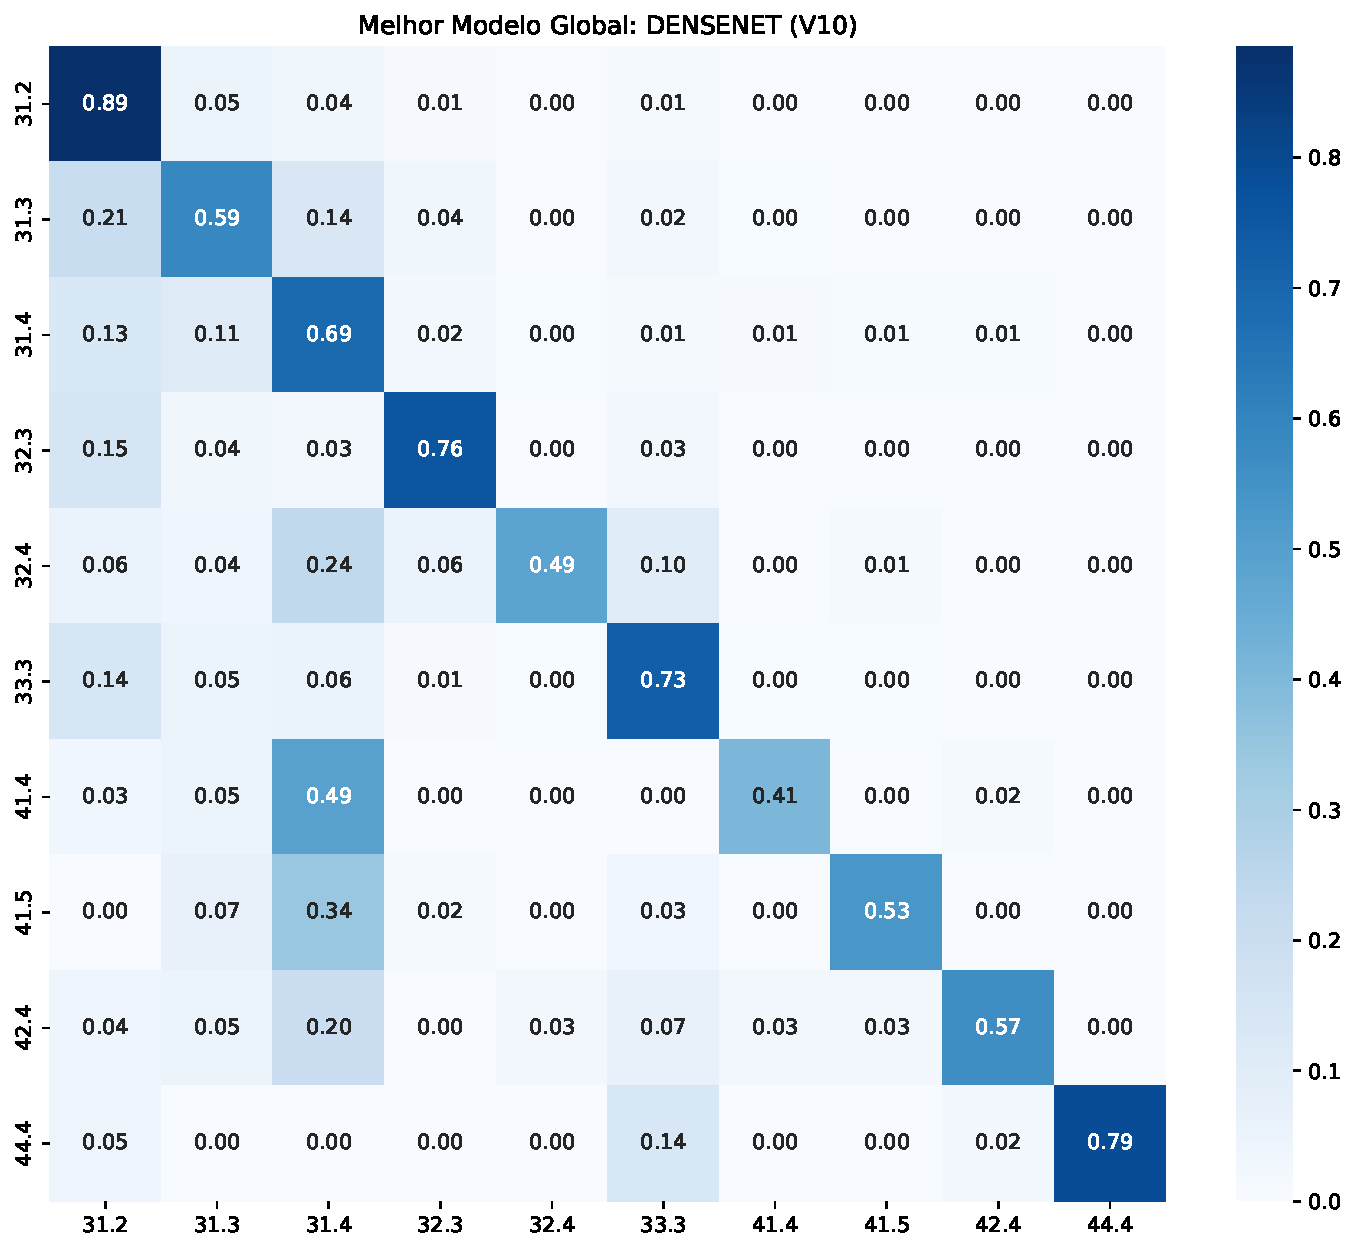
\includegraphics[width=0.9\textwidth]{images/best_model_confusion_matrix.pdf}
  \caption{Matriz de confusão normalizada do modelo DenseNet V10 no conjunto de teste.}
  \label{fig:matriz_confusao_final}
\end{figure}

A análise da matriz revela que as confusões tendem a se concentrar em classes adjacentes no espaço de classificação visual do algodão. Por exemplo, amostras da classe \textbf{41.4} são frequentemente classificadas como \textbf{31.2} ou \textbf{31.4}. Esse comportamento é consistente com a taxonomia física da fibra, onde as fronteiras entre tipos como ``Branco'' e ``Amarelo'' ou ``Tipo 3'' e ``Tipo 4'' podem apresentar sobreposição morfológica sutil, representando o limite intrínseco de discriminabilidade do dataset.
